\documentclass[a4paper,12pt]{report}

\usepackage{alltt, fancyvrb, url}
\usepackage{graphicx}
\usepackage[utf8]{inputenc}
\usepackage{float}
\usepackage{xcolor}
\usepackage{hyperref}
\usepackage[italian]{babel}

\usepackage[italian]{cleveref}

\title{ChaosJack}

\author{Giulia Bardi, Beatrice Pallotti, Elena Lungu, Evelyn Calandrini}
\date{}

\begin{document}

\maketitle

\tableofcontents

\chapter{Analisi}

\section{Descrizione e requisiti}
Il software ChaosJack va a fondere il gioco classico di Black Jack con le meccaniche strategiche e i modificatori tipici di giochi come Balatro, un incontro tra il Poker classico 
e un videogioco di strategia e "rompicapo". L'obiettivo principale del giocatore è quello di sfidare e vincere sia contro il banco sia contro gli altri giocatori presenti al tavolo. Oltre ai giocatori effettivi saranno presenti dei giocatori bot, che seguiranno le regole di gioco in automatico.
Svolgimento della partita: 
\begin{itemize}
	\item Fase iniziale: Per partecipare, ogni giocatore effettua una puntata base. Il banco distribuisce due carte scoperte a ciascun giocatore e a se stesso (scartando la prima e mostrando la seconda).
	\item Valore delle carte: Le figure valgono 10, l'Asso vale 1 o 11 a discrezione del giocatore, le altre carte mantengono il loro valore nominale.
	\item Turno del giocatore: In base al proprio punteggio, il giocatore può chiedere ulteriori carte ("hit") più volte. Se la somma supera 21, il giocatore sballa ed è fuori dalla partita. Il turno termina quando il giocatore decide di fermarsi ("stand").
	\item Fase di puntata finale : Terminato il turno di tutti i giocatori, è possibile effettuare ulteriori scommesse scegliendo una somma o raddoppiando il precedente(questo solo se si possegono due carte in mano).
	\item Turno del banco: Il banco pesca carte fermandosi obbligatoriamente al raggiungimento di un punteggio pari o superiori a 17. Se il banco supera 21, la vincita è contesa tra i giocatori ancora attivi con il punteggio più alto.
\end{itemize}
Condizioni di vittoria e punteggi :
Essendo un tutti contro tutti, per vincere bisogna battere sia il banco che gli altri giocatori.  A parità di punteggio, vince chi ha meno carte in mano. Se il pareggio persiste tra più giocatori, la vincita viene divisa. La vincita standard raddoppia il piatto. Il raggiungimento del Blackjack triplica il piatto, mentre una mano monocolore fornisce un moltiplicatore bonus.
Inoltre, all'avvio di una partita, il giocatore potrebbe imbattersi in turni "speciali" e carte speciali con vincoli che alterano i punteggi.


\subsubsection{Requisiti funzionali}
\begin{itemize}
	\item Il sistema deve permettere lo svolgimento della logica di base del Blackjack, includendo la distribuzione iniziale delle carte e il loro mescolamento. Inoltre deve garantire le azioni di richiesta delle carte, fermarsi, uscire e puntare.
	\item Il sistema deve calcolare correttamente i punteggi delle mani, gestendo la soglia massima del 21 e le regole specifiche associate alle singole carte.
	\item Il gioco deve applicare automaticamente le alterazioni delle regole durante i turni speciali.
	\item Il software deve gestire i portafogli virtuali (fish) sia del giocatore che del banco, aggiornandoli in base all'esito delle puntate.
\end{itemize}

\subsubsection{Requisiti non funzionali}
\begin{itemize}
	\item L'interfaccia utente deve essere reattiva, restituendo un feedback visivo immediato a ogni azione del giocatore senza ritardi percettibili.
	\item Il sistema deve supportare l'aggiunta futura di nuovi modificatori, turni speciali o regole. 
\end{itemize}


\section{Modello del Dominio}

L'ambiente principale è il tavolo, il quale riunisce tutte le entità coinvolte e scandisce lo svolgimento del gioco. Al tavolo siedono i partecipanti, ovvero il banco, i giocatori e i giocatori bot (i quali seguono logiche autonome). Ciascun partecipante è dotato di un proprio portafoglio di fiches e riceve una mano di carte.
L'intero flusso della partita al tavolo è organizzato in una sequenza di fasi ben distinte (come la puntata iniziale o la fase di gioco). 
All'interno di ogni fase, l'azione si articola nei turni individuali dei partecipanti. Durante le fasi di scommessa, le fiches convergono in un piatto centrale. Le carte vengono fornite da un mazzo, che include sia le carte classiche che speciali.
Infine, specifiche partite possono essere alterate dall'applicazione di modificatori, i quali introducono vincoli temporanei alle regole di base alterando le normali fasi di gioco.

\begin{figure}[H]
	\centering{}
	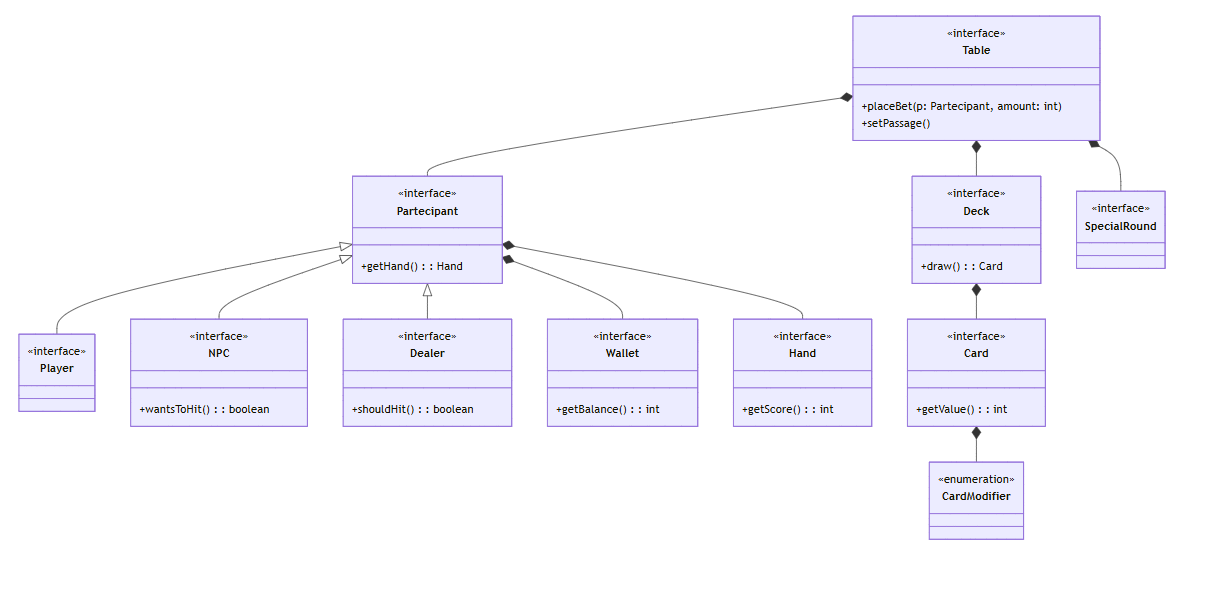
\includegraphics[width=0.8\textwidth]{UML_dominio.png}
	\caption{Schema UML dell'analisi del dominio, con rappresentate le entità principali ed i rapporti fra loro}
	\label{img:analysis}
\end{figure}

\chapter{Design}

\section{Architettura}

L'architettura adottata per il progetto ChaosJack segue il pattern architteturale MVC(Model-View-Controller). Questo pattern consente di avere una chiara separazione delle responsablità e una maggiore flessibilità in fase di sviluppo, permettendoci di separare la logica di gioco dalla sua rappresentazione grafica.
Ovvero è possibile sostituire il blocco della view senza richiedere alcuna modifica nel Controller e nel Model.
L'architettura si basa su queste componenti principali:
\begin{itemize}
	\item Model : GameEngine e Table
	\item Controller : GameFlowController e ActionController
	\item View : ViewManager
\end{itemize}
Il Model : Si occupa di gestire e mantenere in modo consistente lo stato interno del gioco (il mazzo di carte, i portafogli dei partecipanti, il calcolo dei punteggi nelle mani). Valida ed esegue tutte le mutazioni dello stato di gioco secondo le regole tradizionali del BlackJack e l'applicazione dei relativi modificatori speciali.
\\
Il controller : Rappresenta il motore attivo che si occupa di dettare  i tempi e l'ordine delle diverse fasi della partita (regolando i turni tra i giocatori presenti nel tavolo).
\\
La View: Ha il ruolo generale di gestire la visualizzazione dei componenti all'interno della finestra, mostrando l'evoluzione della partita. Si occupa, inoltre, di gestire la fase di navigazione del menù, consentendo di avviare una nuova partita o vedere le statistiche dei round giocati. P

Grazie a questa architettura è possibile sostituire il blocco della view senza richiedere alcuna modifica nel Controller e nel Model.
La View si limita a notificare le azioni dell'utente al Controller. Sarà poi il Controller a invocare i metodi appropriati sul Model per aggiornare lo stato.

\begin{figure}[H]
	\centering{}
	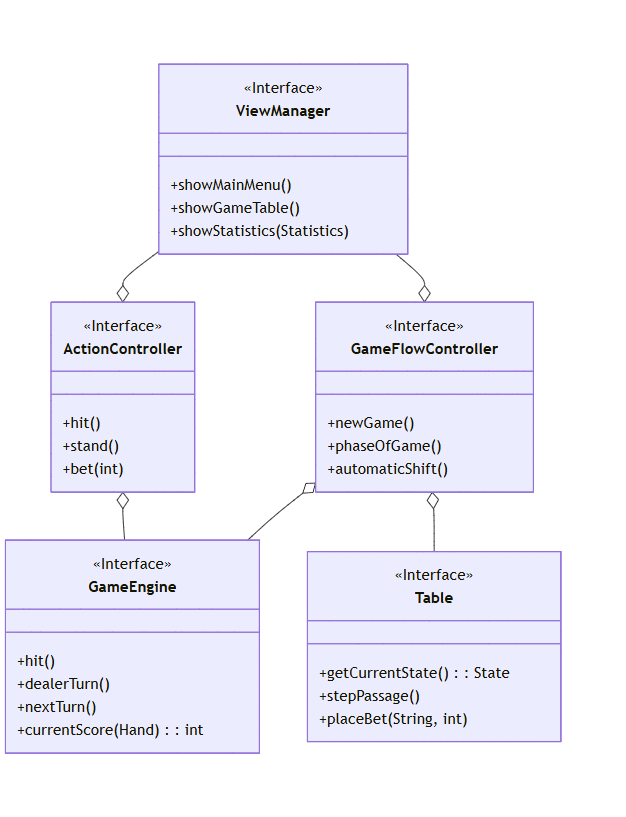
\includegraphics[width=0.8\textwidth]{UML_architettura.png}
	\caption{Schema UML dell'architettura MVC realizzata per ChaosJack}
	\label{img:architettura}
\end{figure}



\section{Design dettagliato}



\subsection*{Evelyn Calandrini - Gestione del Tavolo, Valutazione dei Round, Statistiche, View}
Il contributo si è focalizzato sulla definizione del tavolo che si occupa di riunire il gioco (partecipanti, carte e regole di gioco) occupandosi poi alla fine del round di valutare il vincitore della partita. Si aggiornano così le statistiche salvando il risultato della partita. 
Inoltre il contributo va nell'interfaccia con la gestione del cambio di finestra dalla situazione di gioco, menu, pausa e statistiche.

\paragraph{Gestone dello Stato e delle puntate}
\begin{figure}[H]
	\centering{}
	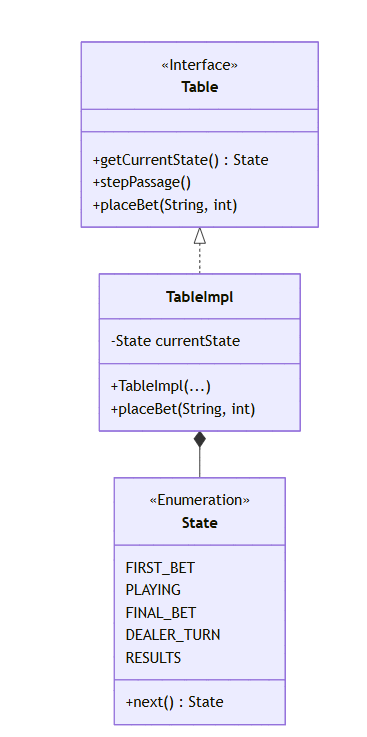
\includegraphics[width=0.3\textwidth]{UML-gestioneStatoTavolo.png}
	\caption{Schema UML rappresenta la gestioni delle fasi di gioco del tavolo}
	\label{img:stato_tavolo}
\end{figure}
\paragraph{Problema} : In un ambiene di gioco a turni, è neccessario garantire che le azione dei singoli giocatori (come effettuare una puntata o chiedere le carte) avvengano esclusivamente nelle fasi corrette di gioco, prevendendo stati inconsistenti o alterazioni 
illecite del piatto.
\\ 
\paragraph{Soluzione} : L'alternativa di usare variabili boolean è stata scarta perchè incline ad errori. Il sistema utilizza un approccio basato su stati di gioco differenziati per le varie fasi di gioco.
Il tavolo (TableImpl) verfica lo stato corrente prima di ogni operazione. In questo modo le varie azione di gioco controllano prima di trovarsi nello stato corretto, se l'azione non è ammessa l'esecuzione viene interrotta.

\paragraph{Valutazione dei risultati}

\begin{figure}[H]
	\centering{}
	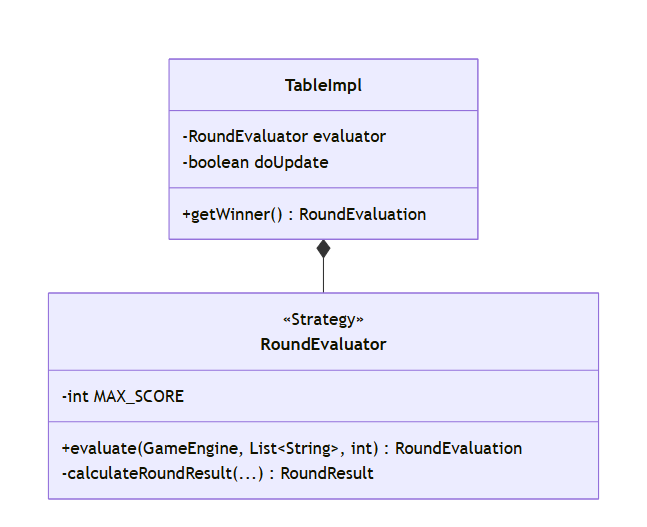
\includegraphics[width=0.3\textwidth]{UML-risultati.png}
	\caption{Schema UML rappresenta l'algoritmo di valutazione (Pattern Strategy)}
	\label{img:valutazione_risultati}
\end{figure}
\paragraph{Problema} : La decratazione del vincitore nel BalckJack richiede la comparazione simultanea dei punteggi di tutti i giocatori contro il banco, tenendo conto delle regole che lo differiscono dal gioco tradizionale (mani monocolore, situazioni di pareggio e turni speciali).
Il problema è fare in modo che il tavolo sia all'oscuro di come sia il calcolo per decretare il vincitore in caso ci sia un cambio di regole futuro.
\\ 
\paragraph{Soluzione} : L'alternativa di implementare il calcolo direttamente all'interno della classe del tavolo è stata scartata, perchè l'avrebbe resa troppo complessa. Si prevede l'isolamento dell'algoritmo di calcolo in una classe esterna RoundEvaluator. Questa classe si occupa di processare lo stato del GameEngine e restiruisce l'esito formattato all'interno del record RoundEvaluation.
In questo modo il tavolo si focalizza sul coordinamento della partita. Facendo così però si ha la necessità di iniettare rifermimenti esterni, come il GameEngine, e il piatto corrente al valutatore ad ogni fine turno. 
La soluzione adotta il pattern Strategy. Il tavolo da gioco delega la strategia per la valutazione del round alla classe RoundEvaluator.

\paragraph{Statistiche e Trasferimento Dati}
\begin{figure}[H]
	\centering{}
	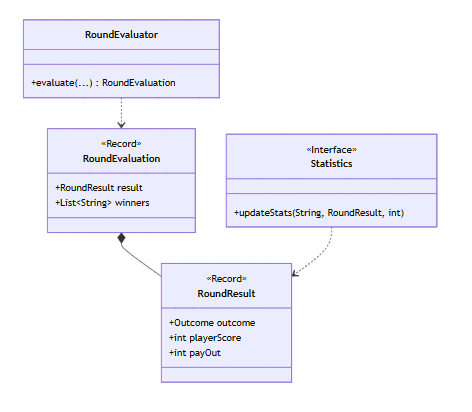
\includegraphics[width=0.3\textwidth]{UML_statistiche.png}
	\caption{Schema UML rappresenta le statistiche e il trasferimento dei dati}
	\label{img:statistiche}
\end{figure}
\paragraph{Problema} : Al termine di ogni round, è necessario comunicare l'esito della partita (vincitori, payout, punteggi) verso il modulo delle statistiche e verso la View. Il rischio principale era l'esposizione di riferimenti diretti agli oggetti del Model, che avrebbe permesso modifiche accidentali allo stato del gioco dall'esterno.
\paragraph{Soluzione} : Un'alternativa sarebbe stata l'interrogazione diretta dei metodi getter del tavolo da parte dei moduli esterni. Questa soluzione è stata scartata poiché avrebbe creato un forte accoppiamento e la possibilità di manipolare indebitamente i dati del Model. La soluzione adottata utilizza i Record.
I record RoundResult e RoundEvaluation sono intrinsecamente immutabili. Questo garantisce che, una volta generato l'esito della partita, il pacchetto di dati sia protetto da qualsiasi alterazione, anche se comporta l'allocazione di nuove istanze a ogni round.
La soluzione utilizza il pattern Data Transfer Object (DTO). I record agiscono come contenitori passivi, trasportando informazioni dal Model verso i restanti componenti del sistema in modo isolato e non modificabile, eliminando qualsiasi dipendenza logica tra chi produce il dato e chi lo consuma.

\paragraph{Gestione dell'Interfaccia (ViewManager)}
\begin{figure}[H]
	\centering{}
	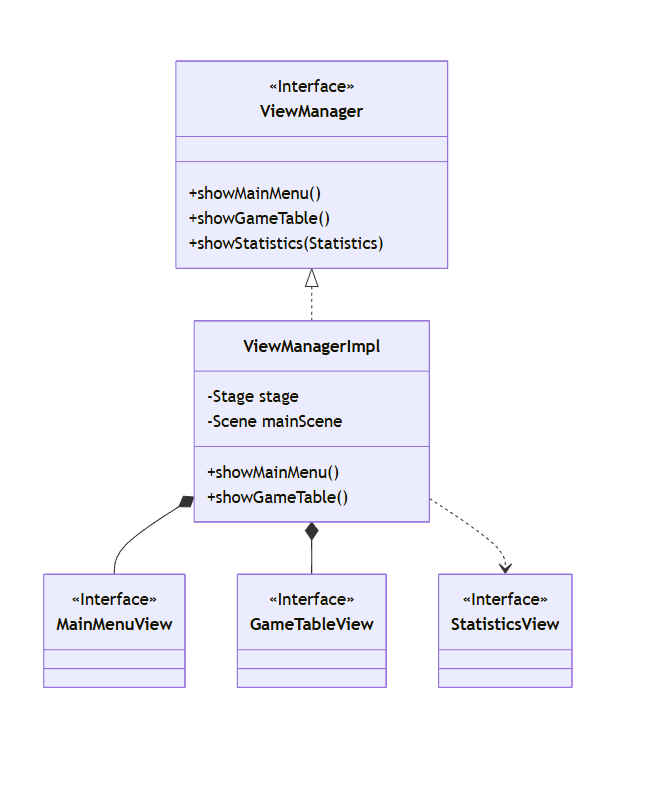
\includegraphics[width=0.3\textwidth]{UML_view.png}
	\caption{Schema UML che rappresenta il ViewManager (Pattern Facade)}
	\label{img:view_manager}
\end{figure}
\paragraph{Problema} : Si prevedono diverse schermate grafiche (Menu, Tavolo di Gioco, Statistiche, Pausa). 
Gestire la transizione tra le scene e la pulizia delle finestre distribuendo la logica nei vari Controller avrebbe accoppiato irrimediabilmente la logica di gioco alla libreria JavaFX.
\paragraph{Soluzione} : Come soluzione si andrà ad utilizzare un gestore centralizzato, il ViewManager. 
Invece di effettuare chiamate incrociate tra le varie schermate, il Controller interagisce esclusivamente con questa interfaccia unificata.
Il ViewManager si occupa internamente di scambiare i nodi e aggiornare lo Stage principale. 
Questa soluzione reifica il pattern Facade, fornendo un punto di accesso semplificato e isolando i Controller dalle complessità della libreria grafica.

\subsection*{Elena Lungu - Gestione delle carte speciali, dei modificatori, wallet e view}
In questa sezione verranno analizzate le scelte progettuali relative alla modellazione delle carte da gioco e del portafoglio del giocatore, componenti fondamentali per l'esperienza di gioco di ChaosJack.

\paragraph{Gestione delle Carte Speciali e Modificatori}
\begin{figure}[H]
	\centering{}
	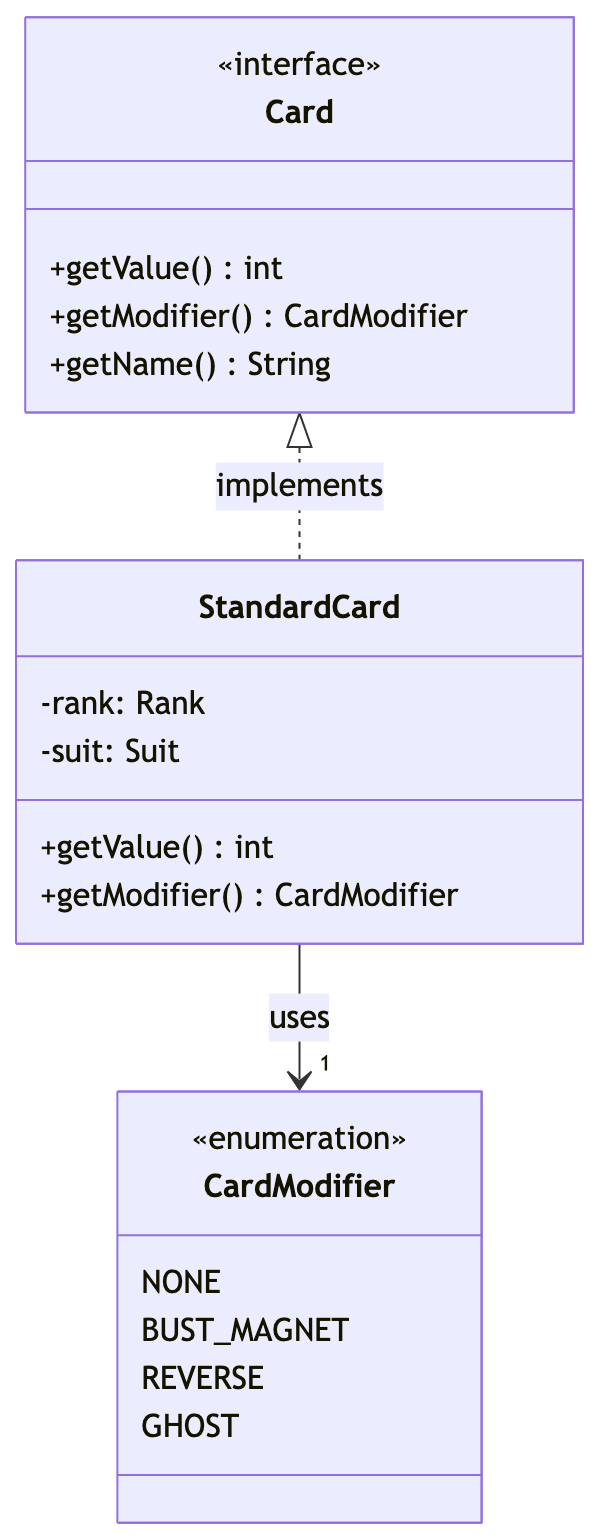
\includegraphics[width=0.45\textwidth]{UML_modificatori.png}
	\caption{Diagramma UML che illustra la relazione tra \texttt{StandardCard} e \texttt{CardModifier}.}
	\label{img:modificatori}
\end{figure}
\paragraph{Problema} : Il gioco ChaosJack introduce la presenza di carte speciali (dette carte "Chaos") che alterano le regole standard del Blackjack, modificando i punteggi o il normale flusso di gioco attraverso l'uso di carte Bust, Reverse, Ghost. Creare una sottoclasse di \texttt{StandardCard} per ogni tipo di carta speciale avrebbe portato a una gerarchia rigida, difficile da mantenere e soggetta a esplosione combinatoria, rendendo complesso aggiungere nuovi effetti in futuro.
\\ 
\paragraph{Soluzione} : Al fine di modellare le carte speciali, si è scelto di applicare il principio fondamentale \textit{"Prefer Composition over Inheritance"}, evitando la creazione di una complessa gerarchia di sottoclassi. È stato introdotto il tipo \texttt{CardModifier}, il quale incapsula la logica necessaria ad alterare il valore della carta. In pratica, una \texttt{StandardCard} riceve il proprio modificatore al momento della creazione; da quel momento in poi, ogni volta che viene richiesto il punteggio della carta, quest'ultima si limita a delegare il calcolo direttamente al suo modificatore.

Questa scelta progettuale è risultata nettamente superiore all'uso dell'ereditarietà per tre motivi principali:
\begin{enumerate}
	\item \textbf{Evita la Class Explosion}: L'uso dell'ereditarietà avrebbe richiesto la creazione di una sottoclasse per ogni singolo effetto (es. \texttt{BustCard}, \texttt{ReverseCard}, \texttt{GhostCard}). In presenza di numerose carte "Chaos", il numero di classi del dominio sarebbe diventato altissimo, rendendo la base di codice difficile da gestire.
	\item \textbf{Rispetta il Principio Open/Closed}: Il sistema è aperto all'estensione ma chiuso alla modifica. Nuovi modificatori possono essere introdotti semplicemente aggiungendo elementi all'enumerazione, lasciando totalmente invariata la logica interna della classe \texttt{StandardCard}.
	\item \textbf{Garantisce flessibilità per future combinazioni}: L'ereditarietà in Java è singola e statica, il che renderebbe impossibile applicare più effetti contemporaneamente senza ricorrere a classi duplicate. Con la composizione, l'architettura è già predisposta per evolvere verso una \texttt{List<CardModifier>} all'interno di \texttt{StandardCard}, permettendo di iterare e applicare combinazioni illimitate di effetti con estrema scalabilità.
\end{enumerate}

La soluzione messa in campo rappresenta un'applicazione del pattern \textit{Strategy}. Invece di definire il comportamento del calcolo del punteggio staticamente all'interno della classe, la \texttt{StandardCard} (che agisce come \textit{Context}) delega il calcolo del suo valore finale al \texttt{CardModifier} che le è stato iniettato.

\paragraph{Disaccoppiamento e Rappresentazione del Wallet (View)}
\begin{figure}[H]
	\centering{}
	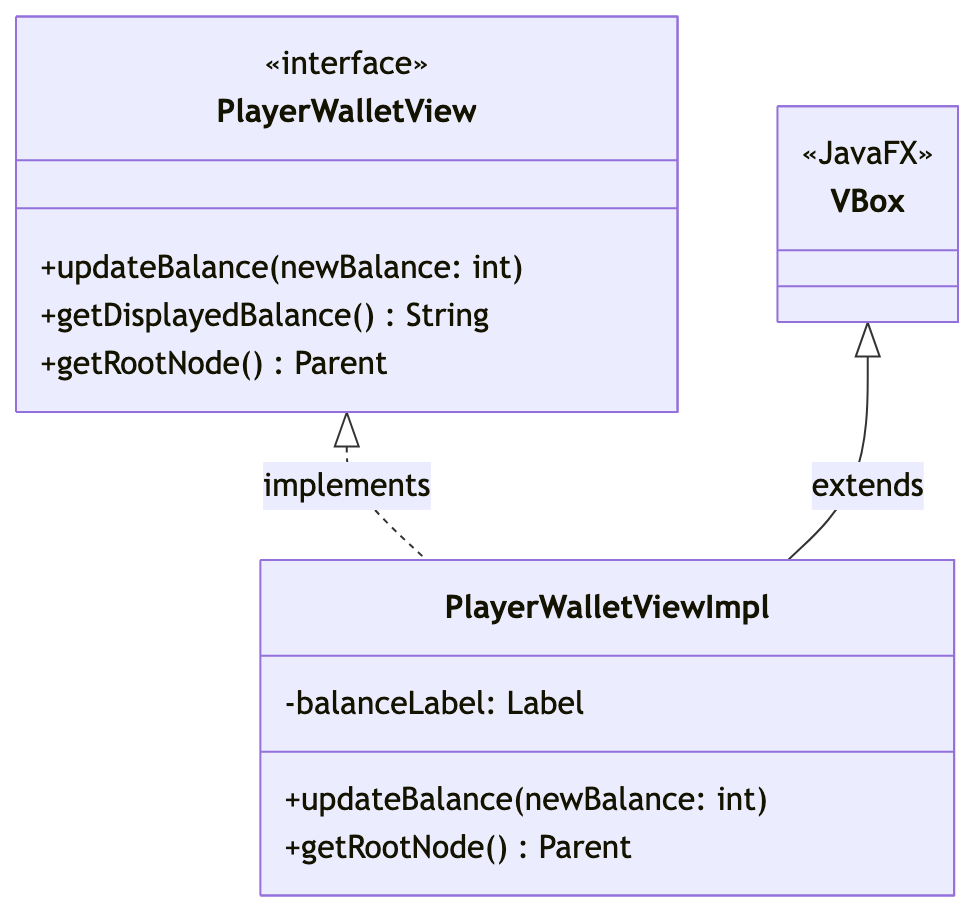
\includegraphics[width=0.45\textwidth]{UML_walletview.png}
	\caption{Diagramma UML che mostra l'incapsulamento della logica grafica in \texttt{PlayerWalletViewImpl}.}
	\label{img:walletview}
\end{figure}
\paragraph{Problema} : Durante la partita, il giocatore deve avere costantemente sotto controllo il proprio saldo (fiches). Era necessario creare un'interfaccia utente grafica per il portafoglio che fosse indipendente dalla logica di gestione dei dati (\texttt{StandardWallet}), facilmente aggiornabile in tempo reale, e che garantisse uno stile visivo accattivante senza alterare le altre componenti della GUI.
\\ 
\paragraph{Soluzione} : È stata creata un'interfaccia specifica \texttt{PlayerWalletView} e la sua implementazione \texttt{PlayerWalletViewImpl}, che estende direttamente un componente JavaFX. L'implementazione maschera totalmente i dettagli grafici (come font, bordi colorati e l'effetto \texttt{DropShadow}) esponendo unicamente metodi di alto livello come \texttt{updateBalance(int newBalance)}.

Come alternativa si era inizialmente valutato di inserire la struttura grafica del portafoglio direttamente nel file FXML principale della partita. Tuttavia, si è optato per l'estrazione in un componente JavaFX dedicato per massimizzare la modularità, il riuso e la \textit{Separation of Concerns}. Qualora in futuro il gioco venisse esteso per supportare più giocatori a schermo (es. multiplayer locale), l'attuale design permetterebbe di istanziare molteplici \texttt{PlayerWalletViewImpl} senza alcuna duplicazione di codice. Inoltre, questa scelta mantiene il Controller principale disaccoppiato e pulito, poiché quest'ultimo interagisce con la View del Wallet solo tramite metodi ad alto livello, senza conoscere i dettagli del rendering interno o la gestione dei nodi figli.

Qui emerge chiaramente l'uso architetturale del pattern MVC applicato ai singoli componenti. \texttt{PlayerWalletViewImpl} agisce come View pura: non possiede alcuna logica di gestione dei dati, non calcola le puntate né verifica se il saldo sia sufficiente (compiti di competenza del Model \texttt{StandardWallet}), ma si limita a visualizzare il valore fornito dal Controller tramite il metodo di aggiornamento.

\chapter{Sviluppo}
\section{Testing automatizzato}

Il processo di testing automatizzato del progetto è stato realizzato per assicurare il corretto funzionamento del codice nel tempo, attraverso una suite di test automatici JUnit.
La strategia di verifica si è concentrata esclusivamente sul model e sui controllori di flusso, tralasciando volontariamente la view e il controller.
La suite di test è stata suddivisa nelle seguenti aree funzionali:
\begin{itemize}
	\item \textbf{Test del motore di gioco e tavolo} (\texttt{GameEngineImplTest, TableTest}): I test garantiscono che il ciclo di vita della partita sia corretto, che le transizioni di stato (es. da puntata a gioco) siano valide e che le regole di gioco vengano applicate rigorosamente. 
	Sono stati inclusi test sui "casi critici", basati sulle regole speciali, per verificare che il tavolo risponda correttamente ad input non previsti.
	\item \textbf{Test delle Entità e Logica di Dominio} (\texttt{DealerTest, PlayerTest, HandTest, WalletTest}): Questi test verificano l'integrità delle componenti base. Si è garantito che la somma dei punteggi delle mani (Hand) sia calcolata correttamente (gestendo il valore flessibile dell'Asso, carte speciali e round speciali) e che il portafoglio (Wallet) 
	impedisca transazioni non coperte dal saldo, È stata validata la correttezza del flusso di denaro: il saldo del portafoglio decresce correttamente all'atto della scommessa e viene incrementato in caso di vincita, assicurando che non si verifichino mai saldi negativi o creazione illecita di credito.
	\item \textbf{Test della Logica di Carte e Mazzi} (\texttt{StandardCardTest, StandardDeckTest}) : i test verificano che il mazzo contenga sempre il numero corretto di carte e che la pesca sia casuale e senza duplicati, prevenendo anomalie algoritmiche nella distribuzione.
	\item \textbf{Test delle Statistiche} (\texttt{StatisticsTest}): I test simulano una serie di round con esiti differenti e validano che il contatore finale di vittorie/sconfitte e il bilancio economico siano esatti, garantendo l'assenza di regressioni nei calcoli storici.
\end{itemize}

\section{Note di sviluppo}

Questa sezione, come quella riguardante il design dettagliato va svolta \textbf{singolarmente da ogni membro del gruppo}.
%
Nella prima parte, ciascuno dovrà mostrare degli esempi di codice particolarmente ben realizzati,
che dimostrino proefficienza con funzionalità avanzate del linguaggio e capacità di spingersi oltre le librerie mostrate a lezione.

\begin{itemize}
	\item \textbf{Elencare} (fare un semplice elenco per punti, non un testo!) le feature \textit{avanzate} del linguaggio e dell'ecosistema Java che sono state
utilizzate. Le feature di interesse sono:
	\begin{itemize}
		\item Progettazione con generici, ad esempio costruzione di nuovi tipi generici, e uso di generici bounded.
		L'uso di classi generiche di libreria non è considerato avanzato.
		\item Uso di lambda expressions
		\item Uso di \texttt{Stream}, di \texttt{Optional} o di altri costrutti funzionali
		\item Uso di reflection
		\item Definizione ed uso di nuove annotazioni
		\item Uso del Java Platform Module System
		\item Uso di parti della libreria JDK non spiegate a lezione (networking, compressione, parsing XML, eccetera...)
		\item Uso di librerie di terze parti (incluso JavaFX): Google Guava, Apache Commons...
	\end{itemize}
	\item Si faccia molta attenzione a non scrivere banalità, elencando qui features di tipo ``core'', come le eccezioni, le enumerazioni, o le inner class: nessuna di queste è considerata avanzata.
	\item Per ogni feature avanzata, mostrata, includere:
	\begin{itemize}
		\item Nome della feature
		\item Permalink GitHub al punto nel codice in cui è stata utilizzata
	\end{itemize}
\end{itemize}

In questa sezione, \textit{dopo l'elenco},
vanno menzionati ed attributi con precisione eventuali pezzi di codice ``riadattati'' (o scopiazzati...) da Internet o da altri progetti,
pratica che tolleriamo ma che non raccomandiamo.
%
Si rammenta agli studenti che non è consentito partire da progetti esistenti e procedere per modifiche successive.
%
Si ricorda anche che i docenti hanno in mano strumenti antiplagio piuttosto raffinati e che ``capiscono'' il codice e la storia delle modifiche del progetto,
per cui tecniche banali come cambiare nomi (di classi, metodi, campi, parametri, o variabili locali),
aggiungere o togliere commenti,
oppure riordinare i membri di una classe vengono individuate senza problemi.
%
Le regole del progetto spiegano in dettaglio l'approccio dei docenti verso atti gravi come il plagiarismo.

I pattern di design \textbf{non} vanno messi qui.
%
L'uso di pattern di design (come suggerisce il nome) è un aspetto avanzato di design, non di implementazione,
e non va in questa sezione.

\subsection*{Elementi positivi}

\begin{itemize}
	\item Si elencano gli aspetti avanzati di linguaggio che sono stati impiegati
	\item Si elencano le librerie che sono state utilizzate
	\item Per ciascun elemento, si fornisce un permalink
	\item Ogni permalink fa riferimento ad uno snippet di codice scritto dall'autore della sezione (i docenti verificheranno usando \texttt{git blame})
	\item Se si è utilizzato un particolare algoritmo, se ne cita la fonte originale.
	Ad esempio, se si è usato Mersenne Twister per la generazione di numeri pseudo-random, si cita \cite{mersenne}.
	\item Si identificano parti di codice prese da altri progetti, dal web, o comunque scritte in forma originale da altre persone.
	In tal senso, si ricorda che agli ingegneri non è richiesto di re-inventare la ruota continuamente:
	se si cita debitamente la sorgente è tollerato fare uso di di snippet di codice open source per risolvere velocemente problemi non banali.
	Nel caso in cui si usino snippet di codice di qualità discutibile,
	oltre a menzionarne l'autore originale si invitano gli studenti ad adeguare tali parti di codice agli standard e allo stile del progetto.
	Contestualmente, si fa presente che è largamente meglio fare uso di una libreria che copiarsi pezzi di codice:
	qualora vi sia scelta (e tipicamente c'è), si preferisca la prima via.
\end{itemize}

\subsection*{Elementi negativi}
\begin{itemize}
	\item Si elencano feature core del linguaggio invece di quelle segnalate. Esempi di feature core da non menzionare sono:
    \begin{itemize}
        \item eccezioni;
        \item classi innestate;
        \item enumerazioni;
        \item interfacce.
    \end{itemize}
	\item Si elencano applicazioni di terze parti (peggio se per usarle occorre licenza, e lo studente ne è sprovvisto) che non c'entrano nulla con lo sviluppo, ad esempio:
    \begin{itemize}
        \item Editor di grafica vettoriale come Inkscape o Adobe Illustrator;
        \item Editor di grafica scalare come GIMP o Adobe Photoshop;
        \item Editor di audio come Audacity;
        \item Strumenti di design dell'interfaccia grafica come SceneBuilder: il codice è in ogni caso inteso come sviluppato da voi.
    \end{itemize}
	\item Si descrivono aspetti di scarsa rilevanza, o si scende in dettagli inutili.
	\item Sono presenti parti di codice sviluppate originalmente da altri che non vengono debitamente segnalate.
	In tal senso, si ricorda agli studenti che i docenti hanno accesso a tutti i progetti degli anni passati,
	a Stack Overflow,
	ai principali blog di sviluppatori ed esperti Java,
	ai blog dedicati allo sviluppo di soluzioni e applicazioni
	(inclusi blog dedicati ad Android e allo sviluppo di videogame),
	nonché ai vari GitHub, GitLab, e Bitbucket.
	Conseguentemente, è \emph{molto} conveniente \emph{citare} una fonte ed usarla invece di tentare di spacciare per proprio il lavoro di altri.
	\item Si elencano design pattern
\end{itemize}

\subsection{Esempio}

\subsubsection{Utilizzo della libreria SLF4J}

Utilizzata in vari punti.
Un esempio è \url{https://github.com/AlchemistSimulator/Alchemist/blob/5c17f8b76920c78d955d478864ac1f11508ed9ad/alchemist-swingui/src/main/java/it/unibo/alchemist/boundary/swingui/effect/impl/EffectBuilder.java#L49}

\subsubsection{Utilizzo di \texttt{LoadingCache} dalla libreria Google Guava}

Permalink: \url{https://github.com/AlchemistSimulator/Alchemist/blob/d8a1799027d7d685569e15316a32e6394632ce71/alchemist-incarnation-protelis/src/main/java/it/unibo/alchemist/protelis/AlchemistExecutionContext.java#L141-L143}

\subsubsection{Utilizzo di \texttt{Stream} e lambda expressions}

Usate pervasivamente. Il seguente è un singolo esempio.
Permalink: \url{https://github.com/AlchemistSimulator/Alchemist/blob/d8a1799027d7d685569e15316a32e6394632ce71/alchemist-incarnation-protelis/src/main/java/it/unibo/alchemist/model/ProtelisIncarnation.java#L98-L120}

\subsubsection{Scrittura di metodo generico con parametri contravarianti}

Permalink: \url{https://github.com/AlchemistSimulator/Alchemist/blob/d8a1799027d7d685569e15316a32e6394632ce71/alchemist-incarnation-protelis/src/main/java/it/unibo/alchemist/protelis/AlchemistExecutionContext.java#L141-L143}

\subsubsection{Protezione da corse critiche usando \texttt{Semaphore}}

Permalink: \url{https://github.com/AlchemistSimulator/Alchemist/blob/d8a1799027d7d685569e15316a32e6394632ce71/alchemist-incarnation-protelis/src/main/java/it/unibo/alchemist/model/ProtelisIncarnation.java#L388-L440}


\chapter{Commenti finali}

In quest'ultimo capitolo si tirano le somme del lavoro svolto e si delineano eventuali sviluppi
futuri.

\textit{Nessuna delle informazioni incluse in questo capitolo verrà utilizzata per formulare la valutazione finale}, a meno che non sia assente o manchino delle sezioni obbligatorie.
%
Al fine di evitare pregiudizi involontari, l'intero capitolo verrà letto dai docenti solo dopo aver formulato la valutazione.

\section{Autovalutazione e lavori futuri}

\textbf{È richiesta una sezione per ciascun membro del gruppo, obbligatoriamente}.
%
Ciascuno dovrà autovalutare il proprio lavoro, elencando i punti di forza e di debolezza in quanto prodotto.
Si dovrà anche cercare di descrivere \emph{in modo quanto più obiettivo possibile} il proprio ruolo all'interno del gruppo.
Si ricorda, a tal proposito, che ciascuno studente è responsabile solo della propria sezione: non è un problema se ci sono opinioni contrastanti, a patto che rispecchino effettivamente l'opinione di chi le scrive.
Nel caso in cui si pensasse di portare avanti il progetto, ad esempio perché effettivamente impiegato, o perché sufficientemente ben riuscito da poter esser usato come dimostrazione di esser capaci progettisti, si descriva brevemente verso che direzione portarlo.

\section{Difficoltà incontrate e commenti per i docenti}

Questa sezione, \textbf{opzionale}, può essere utilizzata per segnalare ai docenti eventuali problemi o difficoltà incontrate nel corso o nello svolgimento del progetto, può essere vista come una seconda possibilità di valutare il corso (dopo quella offerta dalle rilevazioni della didattica) avendo anche conoscenza delle modalità e delle difficoltà collegate all'esame, cosa impossibile da fare usando le valutazioni in aula per ovvie ragioni.
%
È possibile che alcuni dei commenti forniti vengano utilizzati per migliorare il corso in futuro: sebbene non andrà a vostro beneficio, potreste fare un favore ai vostri futuri colleghi.
%
Ovviamente \textit{il contenuto della sezione non impatterà il voto finale}.

\appendix
\chapter{Guida utente}

Capitolo in cui si spiega come utilizzare il software. Nel caso in cui il suo uso sia del tutto
banale, tale capitolo può essere omesso.
%
A tal riguardo, si fa presente agli studenti che i docenti non hanno mai utilizzato il software
prima, per cui aspetti che sembrano del tutto banali a chi ha sviluppato l'applicazione possono non
esserlo per chi la usa per la prima volta.
%
Se, ad esempio, per cominciare una partita con un videogioco è necessario premere la barra
spaziatrice, o il tasto ``P'', è necessario che gli studenti lo segnalino.

\subsection*{Elementi positivi}

\begin{itemize}
 \item Si istruisce in modo semplice l'utente sull'uso dell'applicazione, eventualmente facendo uso di schermate e descrizioni.
\end{itemize}

\subsection*{Elementi negativi}
\begin{itemize}
 \item Si descrivono in modo eccessivamente minuzioso tutte le caratteristiche, anche minori, del software in oggetto.
 \item Manca una descrizione che consenta ad un utente qualunque di utilizzare almeno le funzionalità primarie dell'applicativo.
\end{itemize}

\chapter{Esercitazioni di laboratorio}

In questo capitolo ciascuno studente elenca gli esercizi di laboratorio che ha svolto
(se ne ha svolti),
elencando i permalink dei post sul forum dove è avvenuta la consegna.
%
Questa sezione potrebbe essere processata da strumenti automatici,
per cui link a oggetti diversi dal permalink della consegna,
errori nell'email o nel nome del laboratorio possono portare ad ignorare alcune consegne,
si raccomanda la massima precisione.

\section*{Esempio}

\subsection{paolino.paperino@studio.unibo.it}

\begin{itemize}
 \item Laboratorio 04: \url{https://virtuale.unibo.it/mod/forum/discuss.php?d=12345#p123456}
 \item Laboratorio 06: \url{https://virtuale.unibo.it/mod/forum/discuss.php?d=22222#p222222}
 \item Laboratorio 09: \url{https://virtuale.unibo.it/mod/forum/discuss.php?d=99999#p999999}
\end{itemize}

\subsection{paperon.depaperoni@studio.unibo.it}

\begin{itemize}
 \item Laboratorio 04: \url{https://virtuale.unibo.it/mod/forum/discuss.php?d=12345#p123456}
 \item Laboratorio 05: \url{https://virtuale.unibo.it/mod/forum/discuss.php?d=22222#p222222}
 \item Laboratorio 06: \url{https://virtuale.unibo.it/mod/forum/discuss.php?d=99999#p999999}
 \item Laboratorio 07: \url{https://virtuale.unibo.it/mod/forum/discuss.php?d=22222#p222222}
 \item Laboratorio 08: \url{https://virtuale.unibo.it/mod/forum/discuss.php?d=99999#p999999}
 \item Laboratorio 09: \url{https://virtuale.unibo.it/mod/forum/discuss.php?d=22222#p222222}
 \item Laboratorio 10: \url{https://virtuale.unibo.it/mod/forum/discuss.php?d=99999#p999999}
 \item Laboratorio 11: \url{https://virtuale.unibo.it/mod/forum/discuss.php?d=22222#p222222}
\end{itemize}


\bibliographystyle{alpha}
\bibliography{13-template}

\end{document}
